\documentclass[12pt,a4paper]{article}

\usepackage[textwidth=165mm,textheight=240mm, includehead, includefoot, top =1cm, bottom=1cm,nomarginpar]{geometry}
\setlength{\parindent}{0pt}
\setlength{\parskip}{6pt plus 2pt minus 1pt}
\setlength{\emergencystretch}{3em}  % prevent overfull lines

% xetex settings
% \usepackage{fontspec,xltxtra,xunicode}
% \defaultfontfeatures{Mapping=tex-text,Scale=MatchLowercase}
% \setsansfont[Mapping=tex-text,Ligatures={Common}, Numbers={Lining}]{Helvetica Neue}
% \setmainfont[Mapping=tex-text,Ligatures={Common}, Numbers={Lining}]{Times New Roman}
% \usepackage[math-style=TeX]{unicode-math}
% \setmathfont{STIX Two Math}

%\usepackage{graphicx}
% bring in stuff from pandoc


\providecommand{\tightlist}{%
  \setlength{\itemsep}{0pt}\setlength{\parskip}{0pt}}\usepackage{longtable,booktabs,array}
\usepackage{calc} % for calculating minipage widths
% Correct order of tables after \paragraph or \subparagraph
\usepackage{etoolbox}
\makeatletter
\patchcmd\longtable{\par}{\if@noskipsec\mbox{}\fi\par}{}{}
\makeatother
% Allow footnotes in longtable head/foot
\IfFileExists{footnotehyper.sty}{\usepackage{footnotehyper}}{\usepackage{footnote}}
\makesavenoteenv{longtable}
\usepackage{graphicx}
\makeatletter
\def\maxwidth{\ifdim\Gin@nat@width>\linewidth\linewidth\else\Gin@nat@width\fi}
\def\maxheight{\ifdim\Gin@nat@height>\textheight\textheight\else\Gin@nat@height\fi}
\makeatother
% Scale images if necessary, so that they will not overflow the page
% margins by default, and it is still possible to overwrite the defaults
% using explicit options in \includegraphics[width, height, ...]{}
\setkeys{Gin}{width=\maxwidth,height=\maxheight,keepaspectratio}
% Set default figure placement to htbp
\makeatletter
\def\fps@figure{htbp}
\makeatother

\makeatletter
\makeatother
\makeatletter
\makeatother
\makeatletter
\@ifpackageloaded{caption}{}{\usepackage{caption}}
\AtBeginDocument{%
\ifdefined\contentsname
  \renewcommand*\contentsname{Table of contents}
\else
  \newcommand\contentsname{Table of contents}
\fi
\ifdefined\listfigurename
  \renewcommand*\listfigurename{List of Figures}
\else
  \newcommand\listfigurename{List of Figures}
\fi
\ifdefined\listtablename
  \renewcommand*\listtablename{List of Tables}
\else
  \newcommand\listtablename{List of Tables}
\fi
\ifdefined\figurename
  \renewcommand*\figurename{Figure}
\else
  \newcommand\figurename{Figure}
\fi
\ifdefined\tablename
  \renewcommand*\tablename{Table}
\else
  \newcommand\tablename{Table}
\fi
}
\@ifpackageloaded{float}{}{\usepackage{float}}
\floatstyle{ruled}
\@ifundefined{c@chapter}{\newfloat{codelisting}{h}{lop}}{\newfloat{codelisting}{h}{lop}[chapter]}
\floatname{codelisting}{Listing}
\newcommand*\listoflistings{\listof{codelisting}{List of Listings}}
\makeatother
\makeatletter
\@ifpackageloaded{caption}{}{\usepackage{caption}}
\@ifpackageloaded{subcaption}{}{\usepackage{subcaption}}
\makeatother
\makeatletter
\@ifpackageloaded{tcolorbox}{}{\usepackage[many]{tcolorbox}}
\makeatother
\makeatletter
\@ifundefined{shadecolor}{\definecolor{shadecolor}{rgb}{.97, .97, .97}}
\makeatother
\makeatletter
\makeatother


% Times new roman-like
\usepackage{newtxtext,newtxmath}
\usepackage{sourcesanspro} % sans font

\usepackage{bm}

\providecommand{\tightlist}{%
  \setlength{\itemsep}{0pt}\setlength{\parskip}{2pt}}
\setcounter{secnumdepth}{0}

\usepackage{fancyhdr}
\usepackage{lastpage}
\pagestyle{fancy}
\fancyhf{}
  \renewcommand{\headrulewidth}{0pt}%
\fancyhead{} % clear all header fields
\fancyfoot{} % clear all footer fields
\fancyfoot[LE,LO]{\MakeUppercase{murph101}}
\fancyfoot[CO,CE]{Page \textbf{\thepage} of \textbf{\pageref{LastPage}}}

\usepackage[hidelinks]{hyperref}

\usepackage{enumitem}
\setlist[description]{font=\bfseries\rmfamily,leftmargin=3.8cm,
    style=multiline,itemsep=1\baselineskip,parsep=2pt}
\setlist[enumerate]{font=\bfseries\rmfamily,leftmargin=1.2em,itemsep=1\baselineskip,parsep=2pt}

\usepackage{xstring}
% \usepackage{etoolbox}
% \usepackage{ifthen}

% special case 1 mark to be singular
\newcommand*{\rmarkcases}[1]{\IfStrEq{#1}{1}{[#1 mark]}{[#1 marks]}}%

\providecommand{\rmark}[1]{%
\begin{flushright}%
  \textbf{\rmarkcases{#1}}%
\end{flushright}%
}
% inline version if needed
\providecommand{\rmarkinline}[1]{\mbox{~}\hfill\mbox{\textbf{\rmarkcases{#1}}}}

\providecommand{\thisistheend}{\vfill{\hbox to \textwidth{\hfil * * * * * * * * * * * * * * *\hfil}}\vfill}


% blablabla aliases 
\newcommand{\Grad}{\nabla}
\newcommand{\Div}{\nabla\cdot}
\newcommand{\Curl}{\nabla\times}
\newcommand*\Lapl{\mathop{{}\nabla^2}\nolimits}
% \newcommand*\Laplacian{\mathop{{}\Delta}\nolimits} 

% differentials
\newcommand*\dd{\mathop{}\!\mathrm{d}}

% bold stuff
\newcommand{\bnabla}{\bm{\nabla}}

% hat unit vectors
\newcommand{\vecih}{\mathbf{\hat i}}
\newcommand{\vecjh}{\mathbf{\hat j}}
\newcommand{\veckh}{\mathbf{\hat k}}
\newcommand{\vecyh}{\mathbf{\hat y}}
\newcommand{\veczh}{\mathbf{\hat z}}
\newcommand{\vecdh}{\mathbf{\hat{d}}}
\newcommand{\vecrh}{\mathbf{\hat r}}
\newcommand{\vecnh}{\mathbf{\hat n}} 
\newcommand{\vecrhoh}{\bm{\hat \rho}}
\newcommand{\vecth}{\bm{\hat \theta}}
\newcommand{\vecfh}{\bm{\hat \varphi}} 
\newcommand{\vecxh}{\mathbf{\hat x}}

% vectors
\newcommand{\vecd}{\mathbf{d}}
\newcommand{\veck}{\mathbf{k}}
\newcommand{\vecp}{\mathbf{p}}
\newcommand{\vecr}{\mathbf{r}}
\newcommand{\vecs}{\mathbf{s}}
\newcommand{\vecv}{\mathbf{v}}
\newcommand{\vecx}{\mathbf{x}}

\newcommand{\vecP}{\mathbf{P}}
\newcommand{\vecA}{\mathbf{A}}
\newcommand{\vecB}{\mathbf{B}}
\newcommand{\vecS}{\mathbf{S}}
\newcommand{\vecC}{\mathbf{C}}
\newcommand{\vecD}{\mathbf{D}}
\newcommand{\vecE}{\mathbf{E}}
\newcommand{\vecF}{\mathbf{F}}
\newcommand{\vecG}{\mathbf{G}}
\newcommand{\vecH}{\mathbf{H}}
\newcommand{\vecJ}{\mathbf{J}}


\begin{document}
\pagecolor{white}
%
\begin{titlepage}
\thispagestyle{fancy}
\setcounter{page}{1}
\begin{center}
%
%
\parbox[b]{80mm}{
\includegraphics[width=80mm]{figures/vuw-logo.pdf}
}\par\vskip2em
\bfseries\large{EXAMINATIONS -- \MakeUppercase{2023}}\\
\bfseries\large{TRIMESTER \MakeUppercase{2}}\\
\bfseries\large{FRONT PAGE}\\[2em]
\setlength{\fboxrule}{1pt}\setlength{\fboxsep}{1em}
\framebox{%
\begin{minipage}{80mm}\centering
\MakeUppercase{murph101}\\[0.5em]	% e.g. {COMP 102}
\MakeUppercase{scientific basis of\\
murphy's laws}\\[0.5em]	
\MakeUppercase{Oct 1, 2023}
\end{minipage}}
%
\vspace{3\baselineskip}
\end{center}
%
\begin{description}
  \item[Time allowed:] {\bfseries \MakeUppercase{three hours}}
  \item[Permitted materials:] {\bfseries \MakeUppercase{open book}}\\
  Any materials except communication via electronic devices.
  \item[Instructions:] 
  Attempt ALL \textbf{5} questions

  The exam will be marked out of a total of \textbf{20} marks.

  You can use the formulas listed at the end without rederiving them,\\
  unless explicitly requested.
\end{description}
%
\end{titlepage}

\newpage % First question must not start on front page

\setcounter{page}{2} % titlepage messed with numbers
\hypertarget{first-section}{%
\subsection{FIRST SECTION}\label{first-section}}

\begin{enumerate}
\def\labelenumi{\arabic{enumi}.}
\item
  Multiple choice questions. Briefly justify your answer if unsure.

  \begin{enumerate}
  \tightlist
  \item
    The reflectance of a planar multilayer structure increases with the
    addition of a metal layer:

    \begin{enumerate}
    \tightlist
    \item
      only if placed in front
    \item
      only if placed behind
    \item
      it depends on the structure
    \end{enumerate}
  \item
    At the Brewster angle,

    \begin{enumerate}
    \tightlist
    \item
      TE-polarised light is fully reflected
    \item
      TM-polarised is fully transmitted
    \item
      the transmitted wave is evanescent
    \end{enumerate}
  \item
    A light ray propagating between points A and B in a medium with
    inhomogeneous but isotropic refractive index

    \begin{enumerate}
    \tightlist
    \item
      finds the shortest distance between A and B
    \item
      finds the extremum travel time between A and B
    \item
      has a different trajectory depending on the light polarisation
      \rmark{8}
    \end{enumerate}
  \end{enumerate}
\item
  Solving the Laplace equation.

  \begin{enumerate}
  \tightlist
  \item
    Describe the key steps involved in the method of separation of
    variables for solving the Laplace equation in 3 dimensions.
  \item
    How does the choice of a coordinate system affect the derivation?
    \rmark{5}
  \end{enumerate}
\item
  Question text.\\
  Maybe some extra lines, etc.

  \begin{figure}

  {\centering 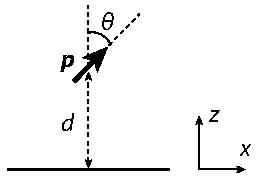
\includegraphics[width=0.4\textwidth,height=\textheight]{figures/schematic.pdf}

  }

  \end{figure}

  Maybe some more lines, etc. \rmark{2}
\item
  Derive the following expressions in spherical coordinates.
  \[\begin{aligned}
  \Grad f={}& \frac{\partial f }{\partial r} \vecrh + 
            \frac{1}{r}\frac{\partial f}{\partial \theta} \vecth +
             \frac{1}{r\sin \theta} \frac{\partial f}{\partial \varphi} \vecfh\\[1pt]
  \Div\vecA ={}&\frac {1}{r^{2}}  \frac{\partial}{\partial r} \left(r^{2}A_{r}\right)+ \frac {1}{r\sin \theta }\frac{\partial}{\partial \theta }\left(\sin \theta A_{\theta }\right)+ \frac {1}{r\sin \theta } \frac{\partial A_{\varphi }}{\partial \varphi }\\[1pt]
  \Curl \vecA ={}& \frac {1}{r\sin \theta } \left(\frac{\partial}{\partial \theta }\left(A_{\varphi }\sin \theta \right)-\frac{\partial A_{\theta }}{\partial \varphi }\right)\vecrh\\[1pt]
  &{}+\frac {1}{r} \left(\frac {1}{\sin \theta } \frac{\partial A_{r}}{\partial \varphi }-\frac{\partial }{\partial r }\left(r A_{\varphi}\right)\right)\vecth\\[1pt] 
  &{}+\frac {1}{r} \left(\frac{\partial }{\partial r }\left(r A_{\theta}\right) - \frac{\partial A_{r}}{\partial \theta }\right)\vecfh\\[1pt]
  \Lapl f={}& \frac {1}{r^2} \frac{\partial }{\partial r} \left(r^{2}\frac{\partial f }{\partial r} \right) + \frac {1}{r^2\sin \theta } \frac{\partial }{\partial\theta } \left(\sin \theta \frac{\partial f}{\partial \theta }\right) + \frac {1}{r^2\sin^2 \theta }\frac{\partial^2 f }{\partial\varphi ^2}
  \end{aligned}\] \rmark{1}
\end{enumerate}

\thisistheend
\pagebreak

\hypertarget{appendix-misc.-formulas-from-the-lecture-notes}{%
\subsection{APPENDIX: Misc. formulas from the lecture
notes}\label{appendix-misc.-formulas-from-the-lecture-notes}}

\hypertarget{vector-calculus-identities}{%
\subsubsection{Vector calculus
identities}\label{vector-calculus-identities}}

\(\Grad (fg) = f\Grad g + g\Grad f\)

\(\Grad (\vecA\cdot\vecB) = \vecA\times(\Curl\vecB) + \vecB\times(\Curl\vecA) + (\vecA\cdot\Grad)\vecB + (\vecB\cdot\Grad)\vecA\)

\(\Div (f\vecA) = f (\Div \vecA) + \vecA\cdot(\Grad f)\)

\(\Div (\vecA\times\vecB) = \vecB\cdot(\Curl\vecA) - \vecA\cdot(\Curl\vecB)\)

\(\Curl (f\vecA) = f(\Curl\vecA) - \vecA\times(\Grad f)\)

\(\Curl (\vecA\times\vecB) = (\vecB\cdot\Grad)\vecA - (\vecA\cdot\Grad)\vecB + (\Div\vecB)\vecA - (\Div\vecA)\vecB\)

\hypertarget{cylindrical-coordinates}{%
\subsubsection{Cylindrical coordinates:}\label{cylindrical-coordinates}}

\(\left\{\begin{aligned} x&=s \cos \varphi \\ y&=s \sin \varphi \\ z&=z \end{aligned}\right.\)

\(\begin{aligned} \Grad f={} & {\frac {\partial f}{\partial s }}{\mathbf {\hat {s }}}+{\frac {1}{s }}{\frac {\partial f}{\partial \varphi }}{\vecfh}+{\frac {\partial f}{\partial z}}\mathbf {\hat {z}} \\[1pt] \Div\vecA ={}&{\frac {1}{s }}{\frac {\partial }{\partial s }}(s A_{s })+{\frac {1}{s }}{\frac {\partial A_{\varphi }}{\partial \varphi }}+{\frac {\partial A_{z}}{\partial z}}\\[1pt] \Curl \vecA ={}& \left({\frac {1}{s }}{\frac {\partial A_{z}}{\partial \varphi }}-{\frac {\partial A_{\varphi }}{\partial z}}\right){\mathbf {\hat {s }}}+\left({\frac {\partial A_{s }}{\partial z}}-{\frac {\partial A_{z}}{\partial s }}\right){\vecfh}+{\frac {1}{s }}\left({\frac {\partial }{\partial s }}(s A_{\varphi })-{\frac {\partial A_{s }}{\partial \varphi }}\right)\mathbf {\hat {z}} \\[1pt] \Lapl f={}& {\frac {1}{s }}{\frac {\partial }{\partial s }}\left(s {\frac {\partial f}{\partial s }}\right)+{\frac {1}{s ^{2}}}{\frac {\partial ^{2}f}{\partial \varphi ^{2}}}+{\frac {\partial ^{2}f}{\partial z^{2}}} \end{aligned}\)

\hypertarget{spherical-coordinates}{%
\subsubsection{Spherical coordinates:}\label{spherical-coordinates}}

\(\left\{\begin{aligned} x&=r\,\sin \theta \,\cos \varphi \\ y&=r\,\sin \theta \,\sin \varphi \\ z&=r\,\cos \theta \end{aligned}\right.\)

\(\begin{aligned} \Grad f={}& \frac{\partial f }{\partial r} \vecrh +  \frac{1}{r}\frac{\partial f}{\partial \theta} \vecth +  \frac{1}{r\sin \theta} \frac{\partial f}{\partial \varphi} \vecfh\\[1pt] \Div\vecA ={}&\frac {1}{r^{2}} \frac{\partial}{\partial r} \left(r^{2}A_{r}\right)+ \frac {1}{r\sin \theta }\frac{\partial}{\partial \theta }\left(\sin \theta A_{\theta }\right)+ \frac {1}{r\sin \theta } \frac{\partial A_{\varphi }}{\partial \varphi }\\[1pt] \Curl \vecA ={}& \frac {1}{r\sin \theta } \left(\frac{\partial}{\partial \theta }\left(A_{\varphi }\sin \theta \right)-\frac{\partial A_{\theta }}{\partial \varphi }\right)\vecrh\\[1pt] &{}+\frac {1}{r} \left(\frac {1}{\sin \theta } \frac{\partial A_{r}}{\partial \varphi }-\frac{\partial }{\partial r }\left(r A_{\varphi}\right)\right)\vecth\\[1pt] &{}+\frac {1}{r} \left(\frac{\partial }{\partial r }\left(r A_{\theta}\right) - \frac{\partial A_{r}}{\partial \theta }\right)\vecfh\\[1pt] \Lapl f={}& \frac {1}{r^2} \frac{\partial }{\partial r} \left(r^{2}\frac{\partial f }{\partial r} \right) + \frac {1}{r^2\sin \theta } \frac{\partial }{\partial\theta } \left(\sin \theta \frac{\partial f}{\partial \theta }\right) + \frac {1}{r^2\sin^2 \theta }\frac{\partial^2 f }{\partial\varphi ^2} \end{aligned}\)

\end{document}
